\subsection{Stability \& Precision} \label{subse:stability_and_precision}

Stability is an important parameter to consider when trying to obtain a solution for nonlinear equations. 
An advantage of the Preissmann scheme is that if the parameter $\theta$ is greater or equal to 0,5, then stability is guaranteed. But guaranteed stability does not necessarily mean precision in the obtained solution. An accurate solution can be found when $\theta$ is set to 0,5 and appropriate values of $\delta t$ and $\delta x$ is chosen. For some explicit schemes utilized for solving the Saint-Venant equations, the Courant number is often used as a stability criterion. It can also be utilized as an indication of precision of the Preissmann scheme. The Courant number can be obtained by the following equation \cite{cunge1980practical, szymkiewicz2010numerical}.

\begin{equation} \label{eq:courant_number_equation}
	C_r =  \frac{\sqrt{g \cdot \overline{\text{H}}} \cdot \Delta t}{\Delta x}
\end{equation}

Where g is the gravitational constant, $\overline{\text{H}}$ is average flow height in the pipe, $\Delta t$ is time step and $\Delta x$ is distance step. A test clarifying the effect of the Courant number is performed on a pipe with the specifications shown in table \ref{tab:pipe_stability_test}.

\begin{table}[H]
\centering
\begin{tabular}{|l|c|}  \hline
Length  	& 500 m \\ \hline
Sections 	& 25  	\\ \hline
$\Delta x$	& 20 m  \\ \hline
Diameter	& 1.2 m \\ \hline
Ib			& 3 \textperthousand \\ \hline
\end{tabular}
\caption{Pipe specifications}
\label{tab:pipe_stability_test}
\end{table}

In the above pipe a step in inflow is given from 0,35 $\text{m}^\text{3}/ \text{s}$ to 0.7 $\text{m}^\text{3}/ \text{s}$. For various Courant numbers, $\Delta t$ is found by equation \ref{eq:courant_number_equation}. The results can be seen in figure \ref{fig:stability_test_theta_0_5}. 

\begin{figure}[H]
 \centering
 % This file was created by matlab2tikz.
%
%The latest updates can be retrieved from
%  http://www.mathworks.com/matlabcentral/fileexchange/22022-matlab2tikz-matlab2tikz
%where you can also make suggestions and rate matlab2tikz.
%
\definecolor{mycolor1}{rgb}{0.00000,0.44700,0.74100}%
\definecolor{mycolor2}{rgb}{0.85000,0.32500,0.09800}%
\definecolor{mycolor3}{rgb}{0.92900,0.69400,0.12500}%
\definecolor{mycolor4}{rgb}{0.49400,0.18400,0.55600}%
\definecolor{mycolor5}{rgb}{0.46600,0.67400,0.18800}%
%
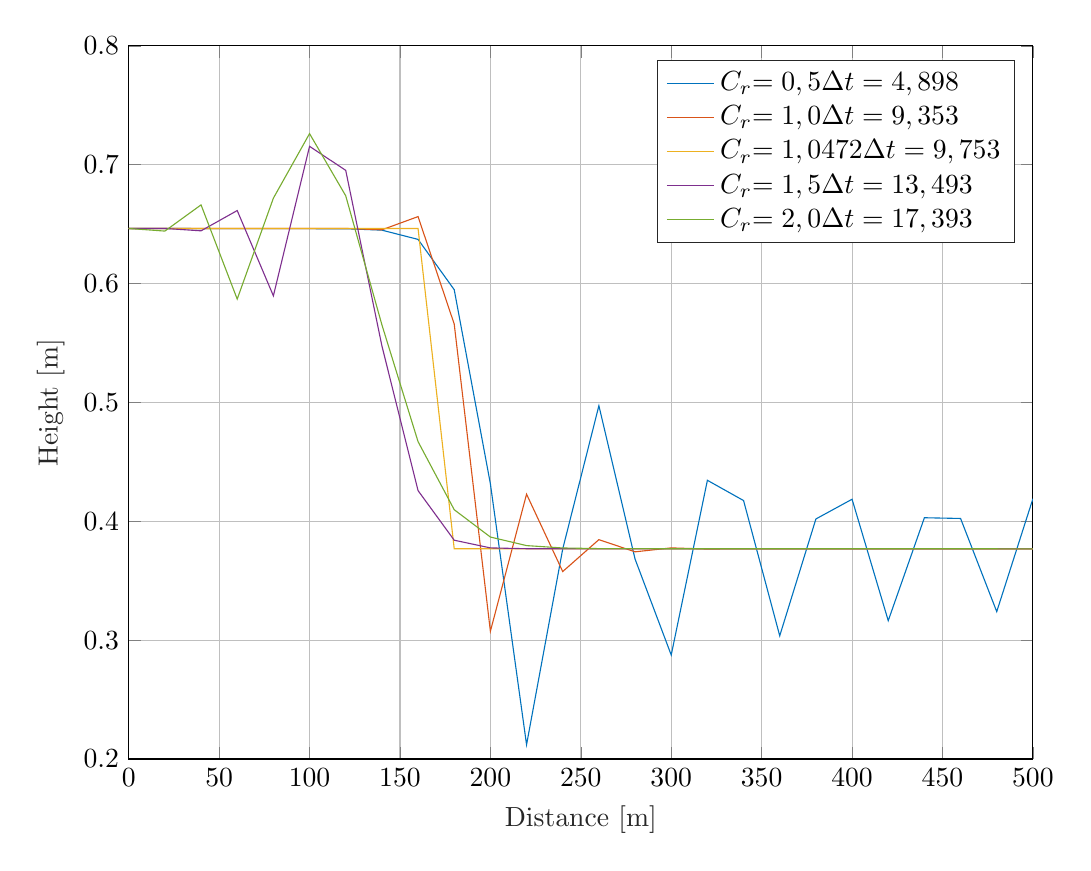
\begin{tikzpicture}

\begin{axis}[%
width=4.521in,
height=3.566in,
at={(0.758in,0.481in)},
scale only axis,
xmin=0,
xmax=500,
xlabel style={font=\color{white!15!black}},
xlabel={Distance [m]},
ymin=0.2,
ymax=0.8,
ylabel style={font=\color{white!15!black}},
ylabel={Height [m]},
axis background/.style={fill=white},
xmajorgrids,
ymajorgrids,
legend style={legend cell align=left, align=left, draw=white!15!black}
]
\addplot [color=mycolor1]
  table[row sep=crcr]{%
0	0.646320000000003\\
120	0.646110798810184\\
140	0.644921440462895\\
160	0.637135852956419\\
180	0.594824492956263\\
200	0.43150901335224\\
220	0.212065679465525\\
240	0.376715133178777\\
260	0.497228602202995\\
280	0.368225074016379\\
300	0.287474004612932\\
320	0.434471939483103\\
340	0.417428829121661\\
360	0.303655446833545\\
380	0.401943487002541\\
400	0.418541170475294\\
420	0.31638041784953\\
440	0.402974501738697\\
460	0.402359479024142\\
480	0.323982099181592\\
500	0.418993270269539\\
};
\addlegendentry{$\text{C}_\text{r}\text{ = 0,5 }\Delta\text{t = 4,898}$}

\addplot [color=mycolor2]
  table[row sep=crcr]{%
0	0.646320000000003\\
100	0.64627269447675\\
120	0.646347802512935\\
140	0.645200955430653\\
160	0.656315606992678\\
180	0.565887713400684\\
200	0.307486457782431\\
220	0.422792612949024\\
240	0.357707826201363\\
260	0.384552559769702\\
280	0.374292850753534\\
300	0.377612917409238\\
320	0.376627578465389\\
340	0.376895037076054\\
420	0.376840400054334\\
500	0.376840417594508\\
};
\addlegendentry{$\text{C}_\text{r}\text{ = 1,0 }\Delta\text{t = 9,353}$}

\addplot [color=mycolor3]
  table[row sep=crcr]{%
0	0.646320000000003\\
120	0.646276927816245\\
160	0.646310155623098\\
180	0.376872286030618\\
360	0.376840417591211\\
500	0.376840417593883\\
};
\addlegendentry{$\text{C}_\text{r}\text{ = 1,0472 }\Delta\text{t = 9,753}$}

\addplot [color=mycolor4]
  table[row sep=crcr]{%
0	0.646320000000003\\
20	0.646369888199388\\
40	0.644339908290192\\
60	0.661409073127913\\
80	0.589657421125025\\
100	0.715402174481824\\
120	0.695236626193719\\
140	0.547617729801175\\
160	0.42579367994415\\
180	0.384067663660119\\
200	0.377602369794033\\
220	0.376914145050648\\
300	0.376840453623174\\
500	0.376840417544031\\
};
\addlegendentry{$\text{C}_\text{r}\text{ = 1,5 }\Delta\text{t = 13,493}$}

\addplot [color=mycolor5]
  table[row sep=crcr]{%
0	0.646320000000003\\
20	0.644131656564412\\
40	0.666181907491705\\
60	0.586925572641576\\
80	0.671829743861394\\
100	0.726113397608458\\
120	0.673833056042724\\
140	0.565341030706179\\
160	0.466990002688476\\
180	0.409725577192091\\
200	0.386732102666656\\
220	0.379534757839167\\
240	0.377540174675403\\
260	0.377017102005198\\
320	0.376843047670491\\
500	0.376840416619302\\
};
\addlegendentry{$\text{C}_\text{r}\text{ = 2,0 }\Delta\text{t = 17,393}$}

\end{axis}
\end{tikzpicture}%
\caption{Step in inflow given from 0,35 $\text{m}^\text{3}/ \text{s}$ to 0.7 $\text{m}^\text{3}/ \text{s}$ at first iteration in pipe listed in table \ref{tab:pipe_stability_test}. Plot for all tests is made at approximately t = 100 seconds.}
\label{fig:stability_test_theta_0_5}
\end{figure}

It is quite clear from the results shown in figure \ref{fig:stability_test_theta_0_5} that considerations should be made when choosing $\Delta t$ and $\Delta x$ as it can have an undesirable effect on the resulting flow. Another anomaly discovered is that the Courant number has to be slightly more than one to obtain a perfect calculation i.e. no oscillation occurring before or after the wave. An attempt to mitigate the error by minimizing the threshold of the approximation by the Newton's method from $10^{-6}$ to $10^{-9}$ yielded no change in the obtained result. Further investigations were not made on the subject.
The parameter $\theta$ should not be left out of the equation, as higher values has a dampening effect on the wave. In figure \ref{fig:stability_theta_test_05_065_1} various values of $\theta$ is tested  with $\delta t$ set to 9,754.    

\begin{figure}[H]
 \centering
 % This file was created by matlab2tikz.
%
%The latest updates can be retrieved from
%  http://www.mathworks.com/matlabcentral/fileexchange/22022-matlab2tikz-matlab2tikz
%where you can also make suggestions and rate matlab2tikz.
%
\definecolor{mycolor1}{rgb}{0.00000,0.44700,0.74100}%
\definecolor{mycolor2}{rgb}{0.85000,0.32500,0.09800}%
\definecolor{mycolor3}{rgb}{0.92900,0.69400,0.12500}%
%

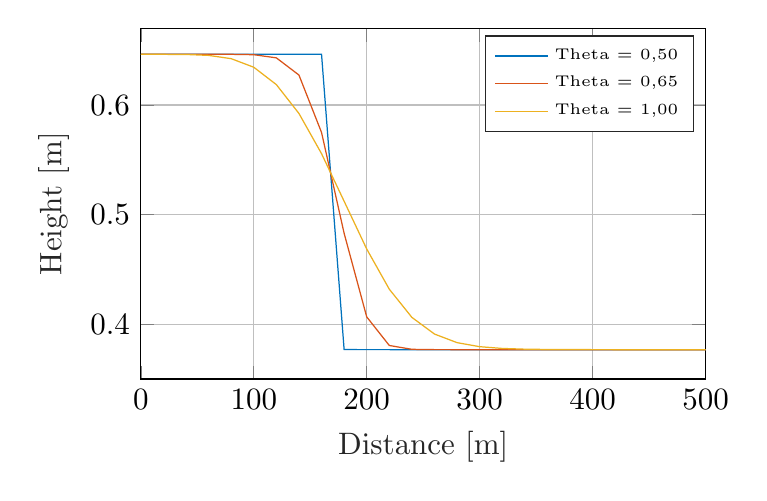
\begin{tikzpicture}[scale=1.12]

\begin{axis}[%
width=2.521in,
height=1.566in,
at={(0.758in,0.481in)},
scale only axis,
xmin=0,
xmax=500,
xlabel style={font=\color{white!15!black}},
xlabel={Distance [m]},
ymin=0.35,
ymax=0.67,
ylabel style={font=\color{white!15!black}},
ylabel={Height [m]},
axis background/.style={fill=white},
xmajorgrids,
ymajorgrids,
legend style={legend cell align=left, align=left, font=\tiny, draw=white!15!black}
]
\addplot [color=mycolor1]
  table[row sep=crcr]{%
0	0.646320000000003\\
60	0.646276050713254\\
160	0.646310155623098\\
180	0.376872286030618\\
280	0.376840431718108\\
500	0.376840417593883\\
};
\addlegendentry{Theta = 0,50}

\addplot [color=mycolor2]
  table[row sep=crcr]{%
0	0.646320000000003\\
80	0.64624640057724\\
100	0.645897528752698\\
120	0.643024844027934\\
140	0.627340662030861\\
160	0.574962749099655\\
180	0.482975200012561\\
200	0.406738255140283\\
220	0.380633403616173\\
240	0.377144178424658\\
260	0.376861538074763\\
400	0.376840417642768\\
500	0.376840417593883\\
};
\addlegendentry{Theta = 0,65}

\addplot [color=mycolor3]
  table[row sep=crcr]{%
0	0.646320000000003\\
40	0.646114001556498\\
60	0.645277732382112\\
80	0.642278908735364\\
100	0.634470248439527\\
120	0.618608579564977\\
140	0.592296821259026\\
160	0.555638802949943\\
180	0.512224654573913\\
200	0.468642227745363\\
220	0.431975238240568\\
240	0.406279099337155\\
260	0.391077260818861\\
280	0.383229133040004\\
300	0.379555033462054\\
320	0.377947501212986\\
340	0.377277301724973\\
360	0.377008073659567\\
400	0.376863443115042\\
500	0.376840600709272\\
};
\addlegendentry{Theta = 1,00}

\end{axis}
\end{tikzpicture}%
\caption{Step in inflow given from 0,35 $\text{m}^\text{3}/ \text{s}$ to 0.7 $\text{m}^\text{3}/ \text{s}$ at first iteration in pipe listed in table \ref{tab:pipe_stability_test}. Plot for all tests is made at approximately t = 97,5 seconds.}
\label{fig:stability_theta_test_05_065_1}
\end{figure}

Due to the choice of simplifying, any natural dampening effect has thereby been disregarded, but as seen in figure \ref{fig:stability_theta_test_05_065_1} artificial dampening due to numerical errors can be reintroduced. By choosing a proper value of $\theta$ the simplification can be somewhat rectified, but at the same time it can mitigate oscillations, which would be bound to happen when pipes of different diameters and slopes is adjoined. As a consequence of introducing numerical dampening, waves of low amplitude will be damped out. But due to the lengths of pipe sewers consists of it is assumed to be an insignificant consequence compared to the reduction in oscillation which can be obtained. According to \cite{cunge1980practical} a value of approximately 0.65 is a reasonable choice for $\theta$, and for that reason it will be used for the remaining part of the project. For comparison the test in figure \ref{fig:stability_test_theta_0_5} is replicated with the chosen value of $\theta$ and can be seen in figure \ref{fig:stability_test_theta_0_65}.

\begin{figure}[H]
 \centering
 % This file was created by matlab2tikz.
%
%The latest updates can be retrieved from
%  http://www.mathworks.com/matlabcentral/fileexchange/22022-matlab2tikz-matlab2tikz
%where you can also make suggestions and rate matlab2tikz.
%
\definecolor{mycolor1}{rgb}{0.00000,0.44700,0.74100}%
\definecolor{mycolor2}{rgb}{0.85000,0.32500,0.09800}%
\definecolor{mycolor3}{rgb}{0.92900,0.69400,0.12500}%
\definecolor{mycolor4}{rgb}{0.49400,0.18400,0.55600}%
\definecolor{mycolor5}{rgb}{0.46600,0.67400,0.18800}%
%

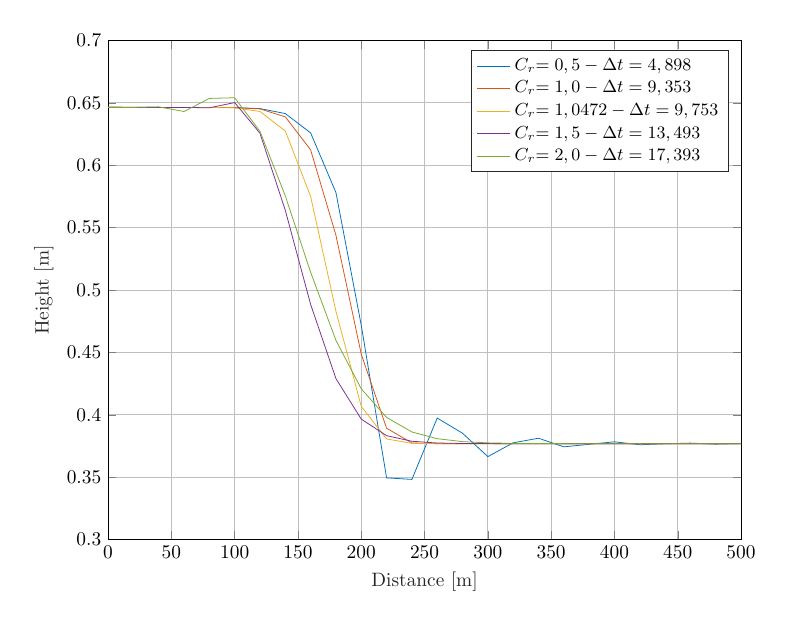
\begin{tikzpicture}[scale=0.7]

\begin{axis}[%
width=4.521in,
height=3.566in,
at={(0.758in,0.481in)},
scale only axis,
xmin=0,
xmax=500,
xlabel style={font=\color{white!15!black}},
xlabel={Distance [m]},
ymin=0.3,
ymax=0.7,
ylabel style={font=\color{white!15!black}},
ylabel={Height [m]},
axis background/.style={fill=white},
xmajorgrids,
ymajorgrids,
legend style={legend cell align=left, align=left, font=\small, draw=white!15!black}
]
\addplot [color=mycolor1]
  table[row sep=crcr]{%
0	0.646320000000003\\
100	0.646130379406088\\
120	0.645319736563408\\
140	0.641349626186809\\
160	0.625859263920574\\
180	0.578058697332551\\
200	0.471670741775881\\
220	0.349470522572005\\
240	0.348227708429135\\
260	0.397395101255427\\
280	0.385197584532591\\
300	0.36649580140255\\
320	0.377549288468572\\
340	0.381224116036606\\
360	0.374323450759618\\
400	0.378357325031061\\
420	0.375997243453128\\
440	0.376767504712859\\
460	0.377314673015633\\
480	0.376460343366603\\
500	0.376957947916708\\
};
\addlegendentry{$\text{C}_\text{r}\text{ = 0,5 } - \Delta\text{t = 4,898}$}

\addplot [color=mycolor2]
  table[row sep=crcr]{%
0	0.646320000000003\\
100	0.646142506713147\\
120	0.645085940723106\\
140	0.638714914649881\\
160	0.612308851353646\\
180	0.543809382353174\\
200	0.448609289609578\\
220	0.389253299316294\\
240	0.377444595181146\\
260	0.376856539679238\\
460	0.376840417593883\\
500	0.376840417593883\\
};
\addlegendentry{$\text{C}_\text{r}\text{ = 1,0 } - \Delta\text{t = 9,353}$}

\addplot [color=mycolor3]
  table[row sep=crcr]{%
0	0.646320000000003\\
80	0.646246242896211\\
100	0.645897359270862\\
120	0.643024752804138\\
140	0.627340728165507\\
160	0.57496313805126\\
180	0.48297580798635\\
200	0.406738381000366\\
220	0.380633284310363\\
240	0.377144123492656\\
260	0.376861434510261\\
420	0.376840417594337\\
500	0.376840417593883\\
};
\addlegendentry{$\text{C}_\text{r}\text{ = 1,0472 } - \Delta\text{t = 9,753}$}

\addplot [color=mycolor4]
  table[row sep=crcr]{%
0	0.646320000000003\\
60	0.646287714980758\\
80	0.645974039633757\\
100	0.650154622142281\\
120	0.625589872774526\\
140	0.563793095912615\\
160	0.488461885784659\\
180	0.42899697304307\\
200	0.396520148575974\\
220	0.383281578277945\\
240	0.378786168330805\\
260	0.377400896181314\\
280	0.376996576980616\\
320	0.376851653469316\\
500	0.376840417670735\\
};

\addlegendentry{$\text{C}_\text{r}\text{ = 1,5 } - \Delta\text{t = 13,493}$}

\addplot [color=mycolor5]
  table[row sep=crcr]{%
0	0.646320000000003\\
20	0.646253446790183\\
40	0.646741328354437\\
60	0.642999942630581\\
80	0.653489860013963\\
100	0.65401950972398\\
120	0.62704350368125\\
140	0.575366566439072\\
160	0.514211327388352\\
180	0.459639658549975\\
200	0.420783611238903\\
220	0.397904618644986\\
240	0.386245066973913\\
260	0.380849107690779\\
280	0.378497038184321\\
300	0.377509898191704\\
320	0.377106256296543\\
360	0.376880597240245\\
500	0.376840457105232\\
};

\addlegendentry{$\text{C}_\text{r}\text{ = 2,0 } - \Delta\text{t = 17,393}$}

\end{axis}
\end{tikzpicture}%
\caption{Step in inflow given from 0,35 $\text{m}^\text{3}/ \text{s}$ to 0.7 $\text{m}^\text{3}/ \text{s}$ at first iteration in pipe listed in table \ref{tab:pipe_stability_test}. Plot for all tests is made at approximately t = 100 seconds.}
\label{fig:stability_test_theta_0_65}
\end{figure}

The chosen value of $\theta$ together with Courant's number as a tuning parameter could be a simple way to obtain values of $\Delta t$ and $\Delta x$ for which less the simulated results is less affected by distortion caused by numerical errors. To be able to conclude on this as a solution further testing would be needed with different pipes with different specifications. Furthermore different steps in inflow would also be needed. Due to the results shown in figure \ref{fig:stability_test_theta_0_65} and time constraints further investigations is not made into the subject.   

%\cite{szymkiewicz2010numerical}